\documentclass{article}
\usepackage{geometry}
\usepackage{graphicx}
\usepackage{float}
\usepackage{subfig}
\usepackage{epsfig}
\usepackage{epstopdf}
\usepackage{amsmath}
\linespread{1.2}



\title{ECS 271 Homework1}
\date{\vspace{-5ex}}
\begin{document}
\author{Jiahui Guan, Leyuan Wang}
\maketitle


\section{PCA}
\subsection{Method Introduction}
A traditional principal component analysis (PCA) is orginally widely used in deep learning (or representation learning). The idea of PCA is to extract the most important features of object (pictures and etc). 

First we need to compare the covariance matrix from the data 
\begin{equation}
\Sigma=\dfrac{1}{m}\sum_{i=1}^m (x^{(i)})(x^{(i)})^T
\end{equation}
Note that $m=624$ as we have total 624 images. $x^{(i)}$ represent each instance and here each instance means each figure. Since each image  here is 64 pixels wide and 60 pixels high, we should have a $64*60$ dimensional data for each instance, that is $x^{(i)}=(x^{(i)})_{1\times 3840}$

\subsection{Deciding the number of features}
Even though the question already states that we need to reduce the dimension to 3, it is good to verify it. To choose the number of important features, which is the reduced dimension, we need to check the eigenvalues of our covariance matrix $\Sigma$ shown in equation (1). Below is the plot of the largest 10 eigenvalues of $\Sigma$. It is clear that the first 3 eigenvalues are much larger than the others meaning that these 3 corresponding features are much more important, so it is reasonable to  reduce dimension to 3-dim using PCA. 
\begin{figure}[H]
\centering
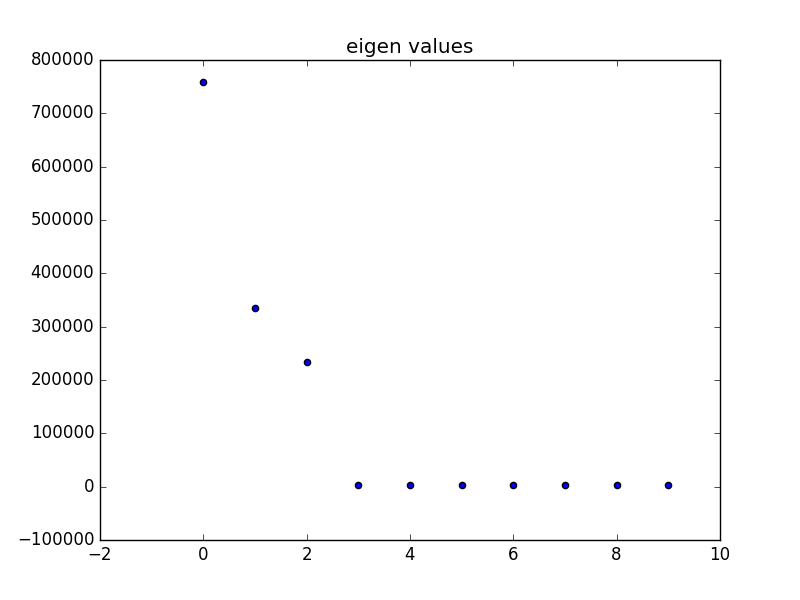
\includegraphics[width=0.6\linewidth, height=6cm]{eigen}
\caption{}
\label{fig:larynx}
\end{figure}


\subsection{Projection vectors}
Before plotting all the instances on the three projection vectors, we first plot the projection vectors, which is the eigenvectors corresponding to the three largest eigenvalues. (See figure 2)
   \begin{figure}[H]
   	\centering
   	
   	\subfloat[]{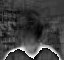
\includegraphics[trim=0cm 0cm 0cm 0cm, clip, width=3.0in]{fig0}}
   	\subfloat[]{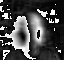
\includegraphics[trim=0cm 0cm 0cm 0cm, clip, width=3.0in]{fig1}}\\
   	\subfloat[]{
\includegraphics[trim=0cm 0cm 0cm 0cm, clip, width=3.0in]{fig2}}
   	\caption{projection vectors corresponding to (a) 1st largest eigenvalue, (b) 2nd largest eigenvalue, (c) third largest eigenvalue}
   	\label{fig:pattern1}
   \end{figure}

\begin{itemize}
\item 1st eigenvalue
We can see that 1 (a), corresponing to 1st largest eigenvalue, represents the color of different people's clothes. Based on the darkness of the color the person wear, it could separate different person. \\

To verify it, we plot all the 624 instances'value on the this projection. Based on the picture below, we can see that there are rougly 20 different ranges of the values, representing 20 different people. \\

Positive value: The pearson wear white(light) cloth\\
Negative value: The pearson wear dark cloth\\

\begin{figure}[H]
\centering
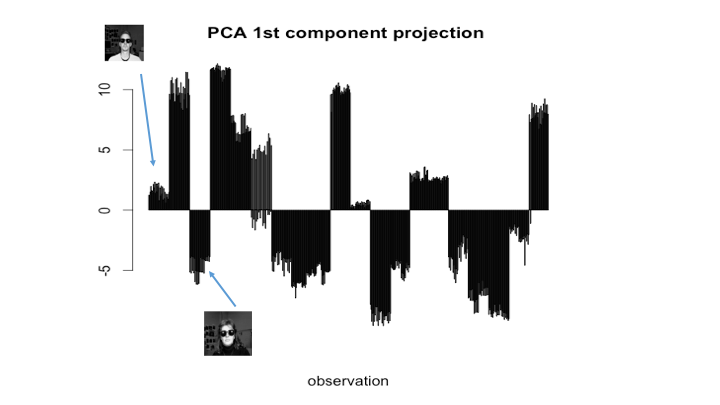
\includegraphics[width=\linewidth, height=8cm]{Slide1}
\caption{}
\label{fig:larynx}
\end{figure}

\item 2nd eigenvalue

Based on figure 2(b), we can see that this projection will determine wether the person turn right and left. To verify it, we plot all the 624 instances'value on the this projection.Based on the picture below, we can see that there are rougly 40 different ranges of the values, representing 20 different people and each with different head directions.\\

Positive value: The pearson turn left\\
Positive value: The pearson turn right\\
\begin{figure}[H]
\centering
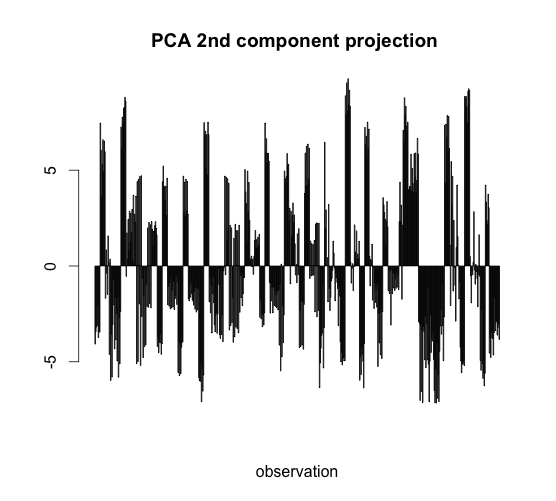
\includegraphics[width=0.8\linewidth, height=8cm]{PCA_figure2}
\caption{}
\label{fig:larynx}
\end{figure}



\item 3rd eigenvalue
It's a bit hard to see what the darker area represent. It might mean that the expression and up-straight of each person. Again, we plot all the instances in this eigenvector (projection). 

\begin{figure}[H]
\centering
\includegraphics[width=0.8\linewidth, height=8cm]{PCA_figure3}
\caption{}
\label{fig:larynx}
\end{figure}


\end{itemize}


\subsection{Scatter plots in 3-dim space}
To put all these three features together, we do a scatter plot for all instances in the 3-dim space.(See figure below).\\

It is somehow hard to see the trend and hard to separate the instances by different people or different poses,expressions etc. But it gives us a broad view of how each instance looks like when we reduce them into a much lower dimensions. Though after dimension reduction, each instance is somehow still separable from each other in 3-dim space.\\

However, there are some spots that are overlapping (those darker spots), meaning that PCA in 3-dim cannot separate them. That leaves room for us to improve this technique. So we use another two methods : LLE and KPCA.

\begin{figure}[H]
\centering
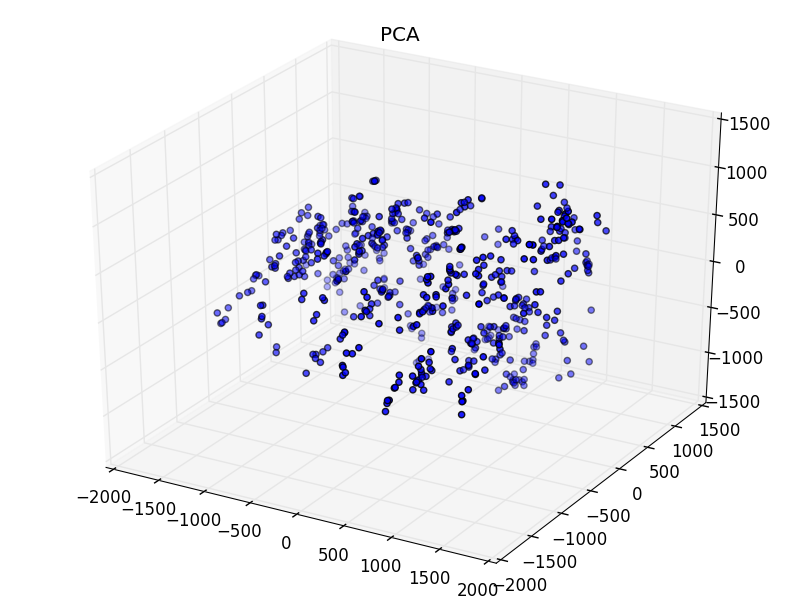
\includegraphics[width=0.8\linewidth, height=8cm]{pca1}
\caption{}
\label{fig:larynx}
\end{figure}

%%%%%%%%%%%%%%%%%%%%%%%%%%%%%%%
\section{LLE}

Locally linear embedding (LLE) is a nonlinear
method for dimensionality reduction and manifold
learning. Given a set of data points distributed on
a manifold in a high dimensional space, LLE is able to
project the data to a lower space by unfolding the 
manifold.[1]\\


The input of the LLE algorithm consists of $n$
dimensional vectors$X_i,i=1,..m (X_i \in  R^n)$.  The
output consists of $d$– dimensional vectors
$Y_i,i=1,...m (Y_i \in  R^d)$. The LLE algorithm has three
steps. In the first step, one identifies neighbours of $X_i$
each data point . Different criteria for neighbour
selection can be adopted; the simplest possibility is to
choose the $k$-nearest neighbours according to the
Euclidean distance. In the second step, one computes
the weights $w_j^i$ that reconstruct each data point $X_i$
best from its neighbours $X_{N(1)},...,X_{N(k)}$ , minimizing
the following error function
\begin{equation}
E(W)=\sum_{i=1}^m |X_i-\sum_{j=1}^k w_j^iX_{N(j)}|
\end{equation}
subject to the constraints $\sum_{j=1}^k w_j^i =1$ and $w_j^i=0$, if $X_i$ and $X_j$ are not neighbours.[1] \\

\subsection{selection of the number of the nearest neighbours}
Since the number $k$ of the nearest neighbours will affect our results, it is essential to check and find the optimal $k$ when implementing LLE. Based on [1], we can a nonparametric correlation Spearman's rho to find the optimal $k$. \\

Computing the distance of orignial data (so each instance will have 3840 dimesions), we can use euclidean distance \[X_{ij}=\sqrt{(x^{(i)}_1-x^{(j)}_1)^2+...+(x^{(i)}_{3840}-x^{(j)}_{3840})^2}\]. Similarily, we can compute the distance of data in reduced dimension (3-dim): \[Y_{ij}=\sqrt{(y^{(i)}_1-y^{(j)}_1)^2+...+(y^{(i)}_3-y^{(j)}_3)^2}\].

Then use Spearman's rho to compute the correlation of $X$ and $Y$. Note that we want to make the correlation as high as possible (highest is 1), which means the two distances in from two different dimensions are similar. 

\begin{equation}
\rho_{spearsman}=1-\dfrac{6\sum_{i=1}^T((r_x(i)-r_y(i))^2}{T^3-T}
\end{equation}

where $r_x(i)$ and $r_y(i)$ are the ranks of the pairwise distances. 

Based on the critieria, we found that $k=30$ will give approximately the largest $\rho$. Thus, we decide to set $k=30$. Figure blow are the scatter plots using LLE with different $k$. You can see that $k=30$ has clearer features' trait than others. 


   \begin{figure}[H]
   	\centering
   	
   	\subfloat[]{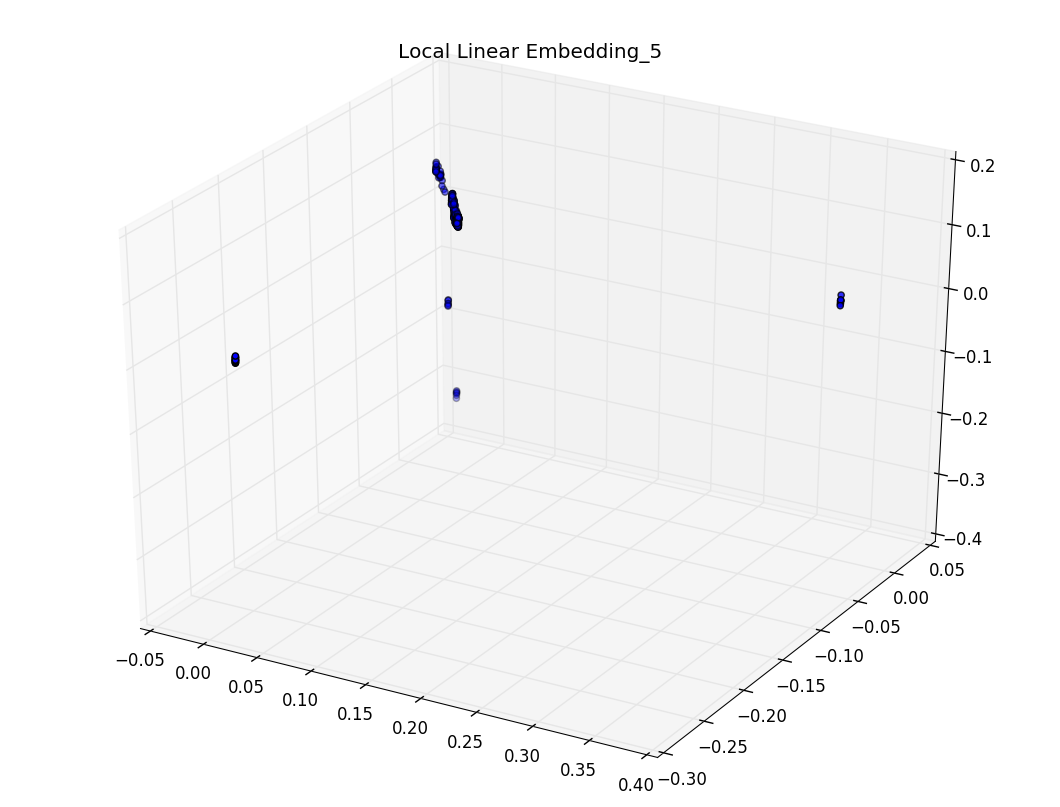
\includegraphics[trim=0cm 0cm 0cm 0cm, clip, width=3.0in]{figure_2}}
   	\subfloat[]{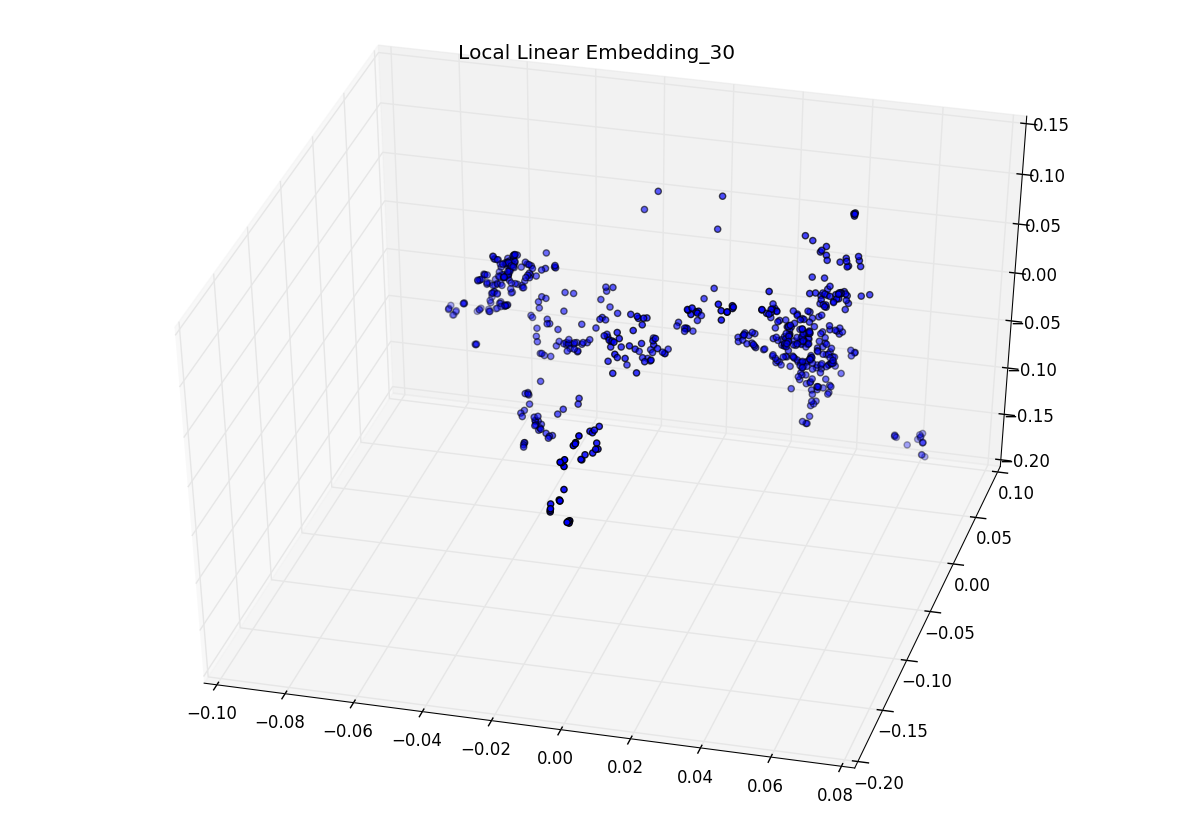
\includegraphics[trim=0cm 0cm 0cm 0cm, clip, width=3.0in]{figure_3}}\\
   	\subfloat[]{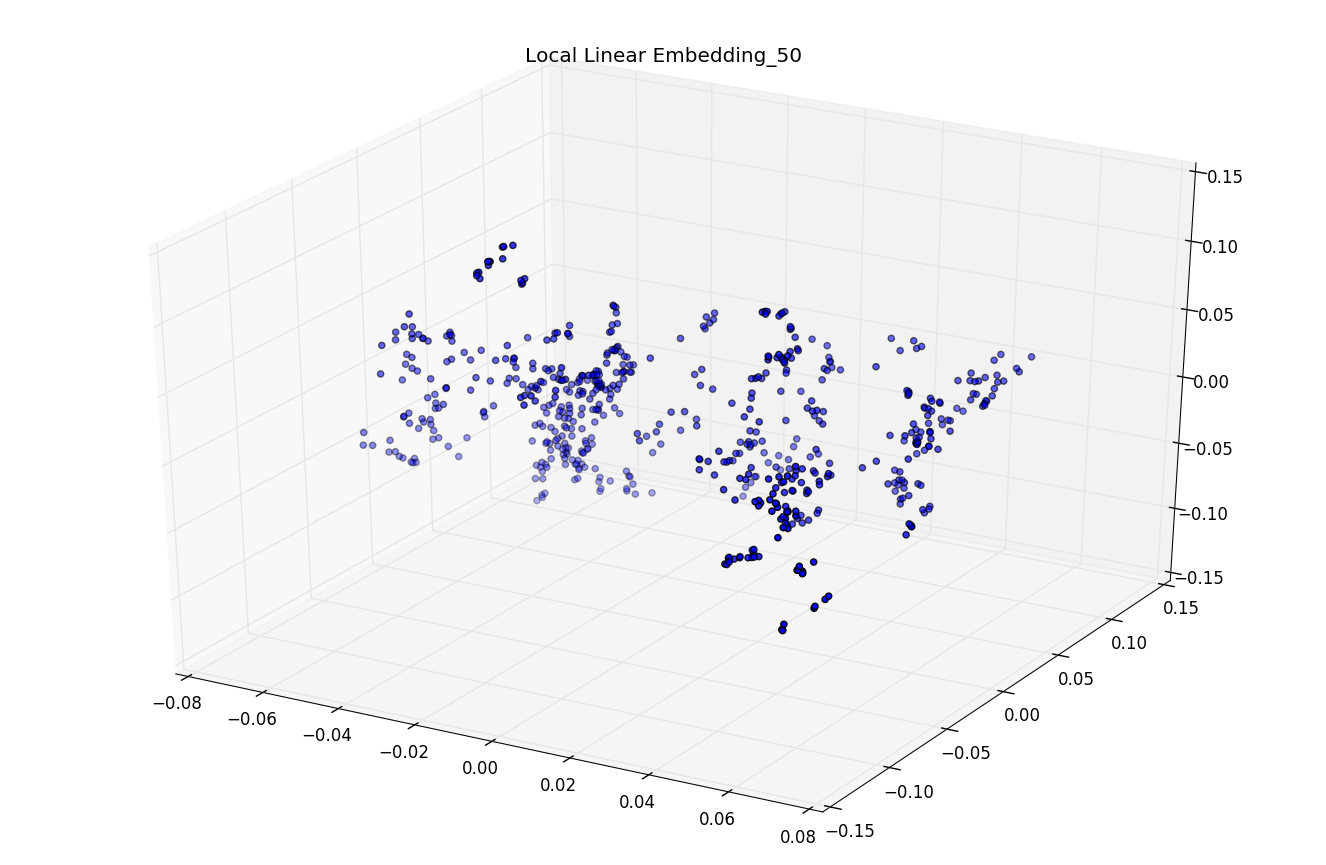
\includegraphics[trim=0cm 0cm 0cm 0cm, clip, width=3.0in]{figure_1}}
   	\caption{scatter plots corresponding to (a) $k=5$, (b) $k=30$, (c) $k=50$}
   	\label{fig:pattern1}
   \end{figure}
\subsection{projection vectors}
Same as what we did in PCA, we also plot all the instances on the three different projection vectors. See figure below. 


\section{KPCA}
Kernelized principal component ananlysis (KPCA) is used when PCA need a kernel to be projected to a higher dimension so that the traits of instances are separable. According to HW1, we can choose different kernels such as linear, polynomial, Guassian and etc. Here based on our numerious experiments, we found that the \textbf{Gaussian Kernel} is better than others.  
 

\end{document}